%!TEX root = ../Topografia_Relazione_MeoliNicola.tex
\chapter{Rototraslazione e variazione di scala}\label{cap:cap3}
Una generica rototraslazione con annessa variazione di unità di misura tra due diversi sistemi di riferimento si effettua mediante:
\begin{equation}
	\label{eq:roto}
	\underline{y}=\mu \mathbf{R} \underline{x}+\underline{t}
\end{equation}
in cui, se le coordinate nei due sistemi di riferimento sono note e se si è nel caso bidimensionale, si possono calcolare i parametri $\mu$,$\alpha$,$t_{(1)}$ e $t_{(2)}$.
Per farlo è opportuno linearizzare i parametri della matrice di rotazione $\mathbf{R}$ sostituendo ai suoi elementi i nuovi parametri $a=\mu\cos\alpha$ e $b=\mu\sin\alpha$:
\[
\mathbf{R}=
\begin{bmatrix}
\cos\alpha & -\sin\alpha \\ 
\sin\alpha & \cos\alpha
\end{bmatrix} 
\quad \Longrightarrow \quad
\mu \mathbf{R} = 
\begin{bmatrix}
a & -b \\ 
b & a
\end{bmatrix} 
\]
\e necessario poi minimizzare la funzione $\Phi$ definita come la somma del vettore degli scarti vettoriali trasposto per lo stesso non trasposto.
\e così possibile stimare i parametri $\hat{a}$ e $\hat{b}$ partendo dalle coordinate iniziali dei punti $k$ $\underline{x_k}$ e $\underline{y_k}$ nei diversi sistemi.
Si calcolano dapprima le media del baricentro:
\begin{align}
\label{eq:media}
\underline{x_B} &= \frac{1}{N}\sum_{k=1}^{N}\underline{x_k}\\
\underline{y_B} &= \frac{1}{N}\sum_{k=1}^{N}\underline{y_k}
\end{align}
per poi calcolare le coordinate baricentriche come differenza tra le coordinate iniziali e la media del baricentro:
\begin{align}
\overline{\underline{x_k}} &= \underline{x_k} - \underline{x_B}\\
\label{eq:baricentriche}
\overline{\underline{y_k}} &= \underline{y_k} - \underline{y_B}
\end{align}
Ridefinendo il vettore $\underline{t}$ come $\underline{t_{0}}=\underline{t}-\underline{w}_{B}+\lambda \mathbf{R} \underline{u}_{B}$ è possibile riportarsi all'equazione \ref{eq:roto} in cui però compaiono le coordinate baricentriche.
\begin{equation}
\underline{y_{k}}=
\begin{bmatrix}
	{a} & {-b} \\ 
	{b} & {a}
\end{bmatrix} 
\overline{x_{k}}+\underline{t_{0}}
\end{equation}
che in forma espansa diventa:
\begin{equation}
	\begin{bmatrix}
		\underline{y}_{k(1)} \\ 
		\underline{y}_{k(2)}
	\end{bmatrix} 
	=
	\begin{bmatrix}
		{a} & {-b} \\ 
		{b} & {a}
	\end{bmatrix}
	\begin{bmatrix}
		\underline{x}_{k(1)} \\ 
		\underline{x}_{k(2)}
	\end{bmatrix}
	+
	\begin{bmatrix}
		\underline{t}_{(1)} \\ 
		\underline{t}_{(2)}
	\end{bmatrix}
\end{equation}
Chiamando il vettore dei termini noti con $\underline{\eta}$, quello dei termini incogniti con $\underline{\xi}$ e con $\mathbf{A}$ la matrice dei coefficienti, si ha:
\begin{equation}
	\underline{\eta}=\mathbf{A} \underline{\xi}
\end{equation}
Si tratta di un sistema facilmente risolvibile se si considerano le coordinate $x$ note senza errori e le coordinate $y$ con pari varianza e non correlate tra loro. 
\begin{equation}
	\hat{\underline{\xi}}=	
	\left(\mathbf{A}^T \mathbf{A}\right)^{-1}
	\left(\mathbf{A}^T \underline{\eta}\right)
\end{equation}
Permette così di trovare i parametri $d$, $p$, $q$, $a$ e $b$:
\begin{align} d &=\sum_{k=1}^{N}\left(\overline{x}_{k(1)}^{2}+\overline{x}_{k(2)}^{2}\right) \\ 
p &=\sum_{k=1}^{N}\left(\overline{x}_{k(1)} \overline{y}_{k(1)}+\overline{x}_{k(2)} \overline{y}_{k(2)}\right) \\ 
q &=\sum_{k=1}^{N}\left(\overline{x}_{k(1)} \overline{y}_{k(2)}-\overline{x}_{k(2)} \overline{y}_{k(1)}\right) \\
\hat{a} &= \frac{p}{d} \\
\hat{b} &= \frac{q}{d}
\end{align}
Grazie ai quali è possibile calcolare le stime $\hat{\mu}$, $\hat{\alpha}$ e il vettore degli scarti $\underline{v}$.
Quest'ultimo ottenuto minimizzando la funzione:
\begin{equation}
	\Phi = \sum_k \underline{v}^T\underline{v}_k
\end{equation}
\begin{align}
	\hat{\mu} &= \sqrt{\hat{a}^2 + \hat{b}^2}\\
	\hat{\alpha} &= \arctan\frac{\hat{b}}{\hat{a}}\\
	\underline{v_k} &= 
	\overline{\underline{y_{k}}}-
	\begin{bmatrix}
		\hat{a} & -\hat{b} \\ 
		\hat{b} & \hat{a}
	\end{bmatrix} 
	\overline{x_{k}} \\
	\hat{\sigma}_0^2 &= \frac{\underline{v_k}^T \,\mathbf{Q} \, \underline{v_k}}{r}=\frac{\underline{v_k}^T \, \mathbf{I} \, \underline{v_k}}{r}
\end{align}
\section{Esempio applicativo}
Si applica ora il metodo appena visto ad un esempio di rototraslazione con i seguenti dati iniziali:
\begin{center}
\begin{tabular}%numeri prima e dopo la virgola per evitare il troppo spazio tra le colonne
		{c%
		S[table-format=1.2]%
		S[table-format=1.2]%
		S[table-format=3.2]%
		S[table-format=3.2]}
\toprule
{$\mathbf{k}$}& {$\mathbf{x_1}$} & {$\mathbf{x_2}$} & {$\mathbf{y_1}$}   & {$\mathbf{y_2}$}   \\ \midrule
$\mathbf{A}$ & 5.00 & 0.00 & 199.96 & 300.00 \\
$\mathbf{B}$ & 5.00 & 5.00 & 100.00 & 400.04 \\
$\mathbf{C}$ & 0.00 & 5.00 & 0.04   & 300.00 \\
$\mathbf{D}$ & 0.00 & 0.00 & 100.00 & 199.96 \\ \bottomrule
\end{tabular}
\end{center}
in cui si calcolano le medie e le coordinate baricentriche con le \eqref{eq:media} - \eqref{eq:baricentriche}:
\begin{align*}
\overline{\underline{x_k}} &= \left(2,50;2,50\right) \\
\overline{\underline{y_k}} &= \left(100,00;300,00\right)
\end{align*}
\begin{center}
\begin{tabular}%numeri prima e dopo la virgola per evitare il troppo spazio tra le colonne
		{c%
		S[table-format=1.2]%
		S[table-format=1.2]%
		S[table-format=2.2]%
		S[table-format=3.2]}
\toprule
{$\mathbf{k}$}& {$\mathbf{x_1}$} & {$\mathbf{x_2}$} & {$\mathbf{y_1}$}   & {$\mathbf{y_2}$}   \\ \midrule
$\mathbf{A}$ & 2.50  & -2.50 & 99.96  & 0.00    \\
$\mathbf{B}$ & 2.50  & 2.50  & 0.00   & 100.04  \\
$\mathbf{C}$ & -2.50 & 2.50  & -99.96 & 0.00    \\
$\mathbf{D}$ & -2.50 & -2.50 & 0.00   & -100.04 \\  \bottomrule
\end{tabular}
\end{center}
\e poi possibile ricavare tutti gli altri parametri visti sopra:
\begin{align*}
	p=\SI{1000.00}{} \qquad &q=\SI{1000.00}{} \\
	d=\SI{50.00}{} \qquad &\hat{a}=\SI{200.00}{} \\
	\hat{b}=\SI{20.00}{} \qquad &\hat{\mu}=\SI{28.28}{} \\
	\hat{\alpha}=\SI{0.785}{^r} \qquad &\hat{\sigma}_0^2=\SI{1.6e-3}{}\\
	\hat{\sigma}_0=\SI{4e-2}{}	\qquad &\hat{\underline{v}}_k=
	\begin{bmatrix}
	-0,04 \\ 
	0 \\ 
	0 \\ 
	0,04 \\ 
	0,04 \\ 
	0 \\ 
	0 \\ 
	-0,04
	\end{bmatrix} 
\end{align*}

Lo stesso esempio è stato rifatto all'interno di un foglio elettronico ottenendo ovviamente gli stessi risultati:
\begin{figure}[H]
\centering
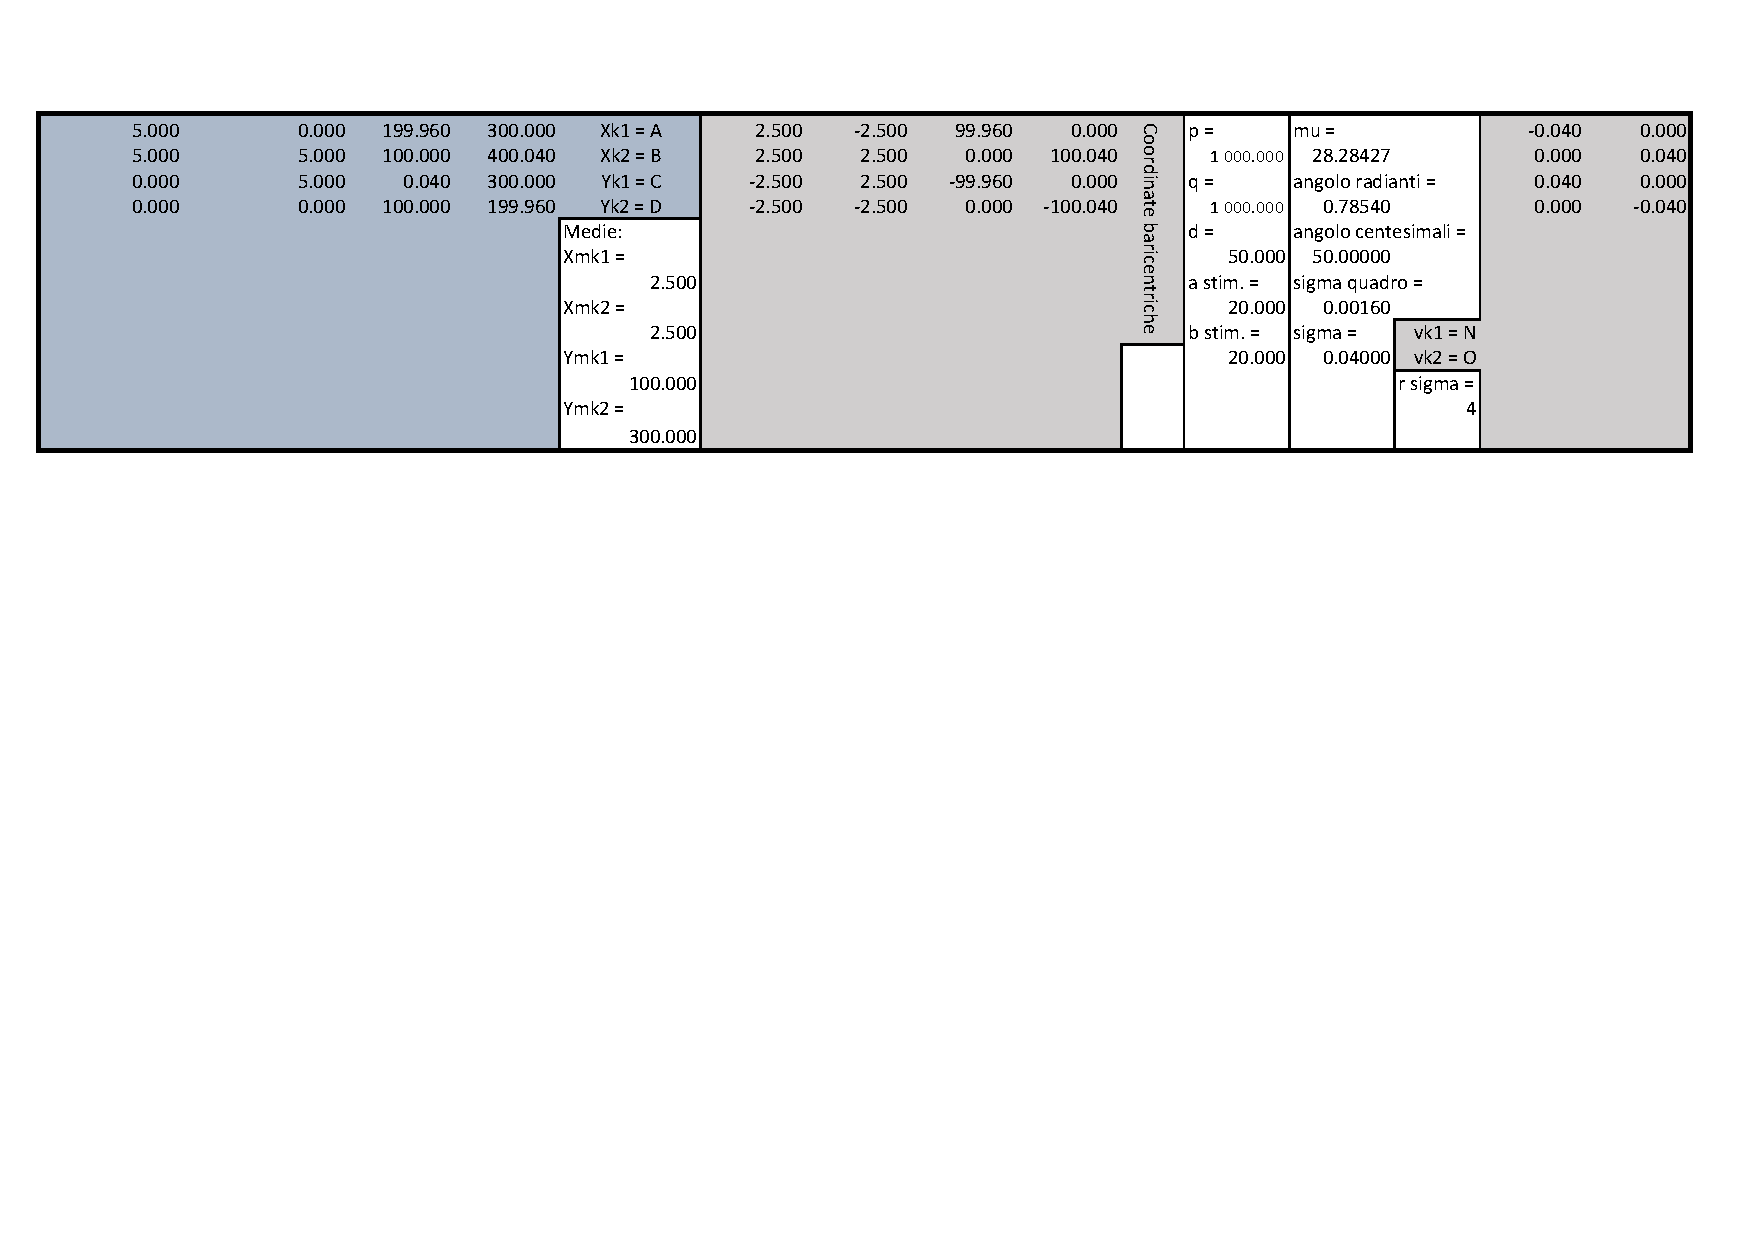
\includegraphics[width=16cm]{documents/rototraslazioneEsempio.pdf}
\caption{Schermata del foglio di calcolo con il quale è stata eseguita la rototraslazione dell'esempio applicativo}
\end{figure}
\section{Rototraslazione ad un rilievo reale}
Il metodo visto ed eseguito in foglio di calcolo lo si applica ora ad un rilievo reale svolto due anni fa con i seguenti dati iniziali:
\begin{center}
\begin{tabular}%numeri prima e dopo la virgola per evitare il troppo spazio tra le colonne
		{c%
		S[table-format=6.3]%
		S[table-format=7.3]%
		S[table-format=2.3]%
		S[table-format=2.3]}
\toprule
{$\mathbf{k}$}& {$\mathbf{x_1}$} & {$\mathbf{x_2}$} & {$\mathbf{y_1}$}   & {$\mathbf{y_2}$}   \\ \midrule
$\mathbf{A}$ & 665 428.996 & 5 103 529.385 & 29.930 & 23.856    \\
$\mathbf{B}$ & 665 392.368 & 5 103 518.312 & 0.000  & 0.000  \\
$\mathbf{C}$ & 665 368.282 & 5 103 455.441 & 0.907  & -67.327    \\
$\mathbf{D}$ & 665 467.836 & 5 103 518.510 & 70.013 & 28.155 \\  \bottomrule
\end{tabular}
\end{center}
Portando ai seguenti risultati finali:
\begin{align*}
	\hat{\mu}&=\SI{1.00007}{}\\
	\hat{\alpha}&=\SI{1.1912}{^r}=\SI{75.8393}{^g}
\end{align*}
\begin{figure}[H]
\centering
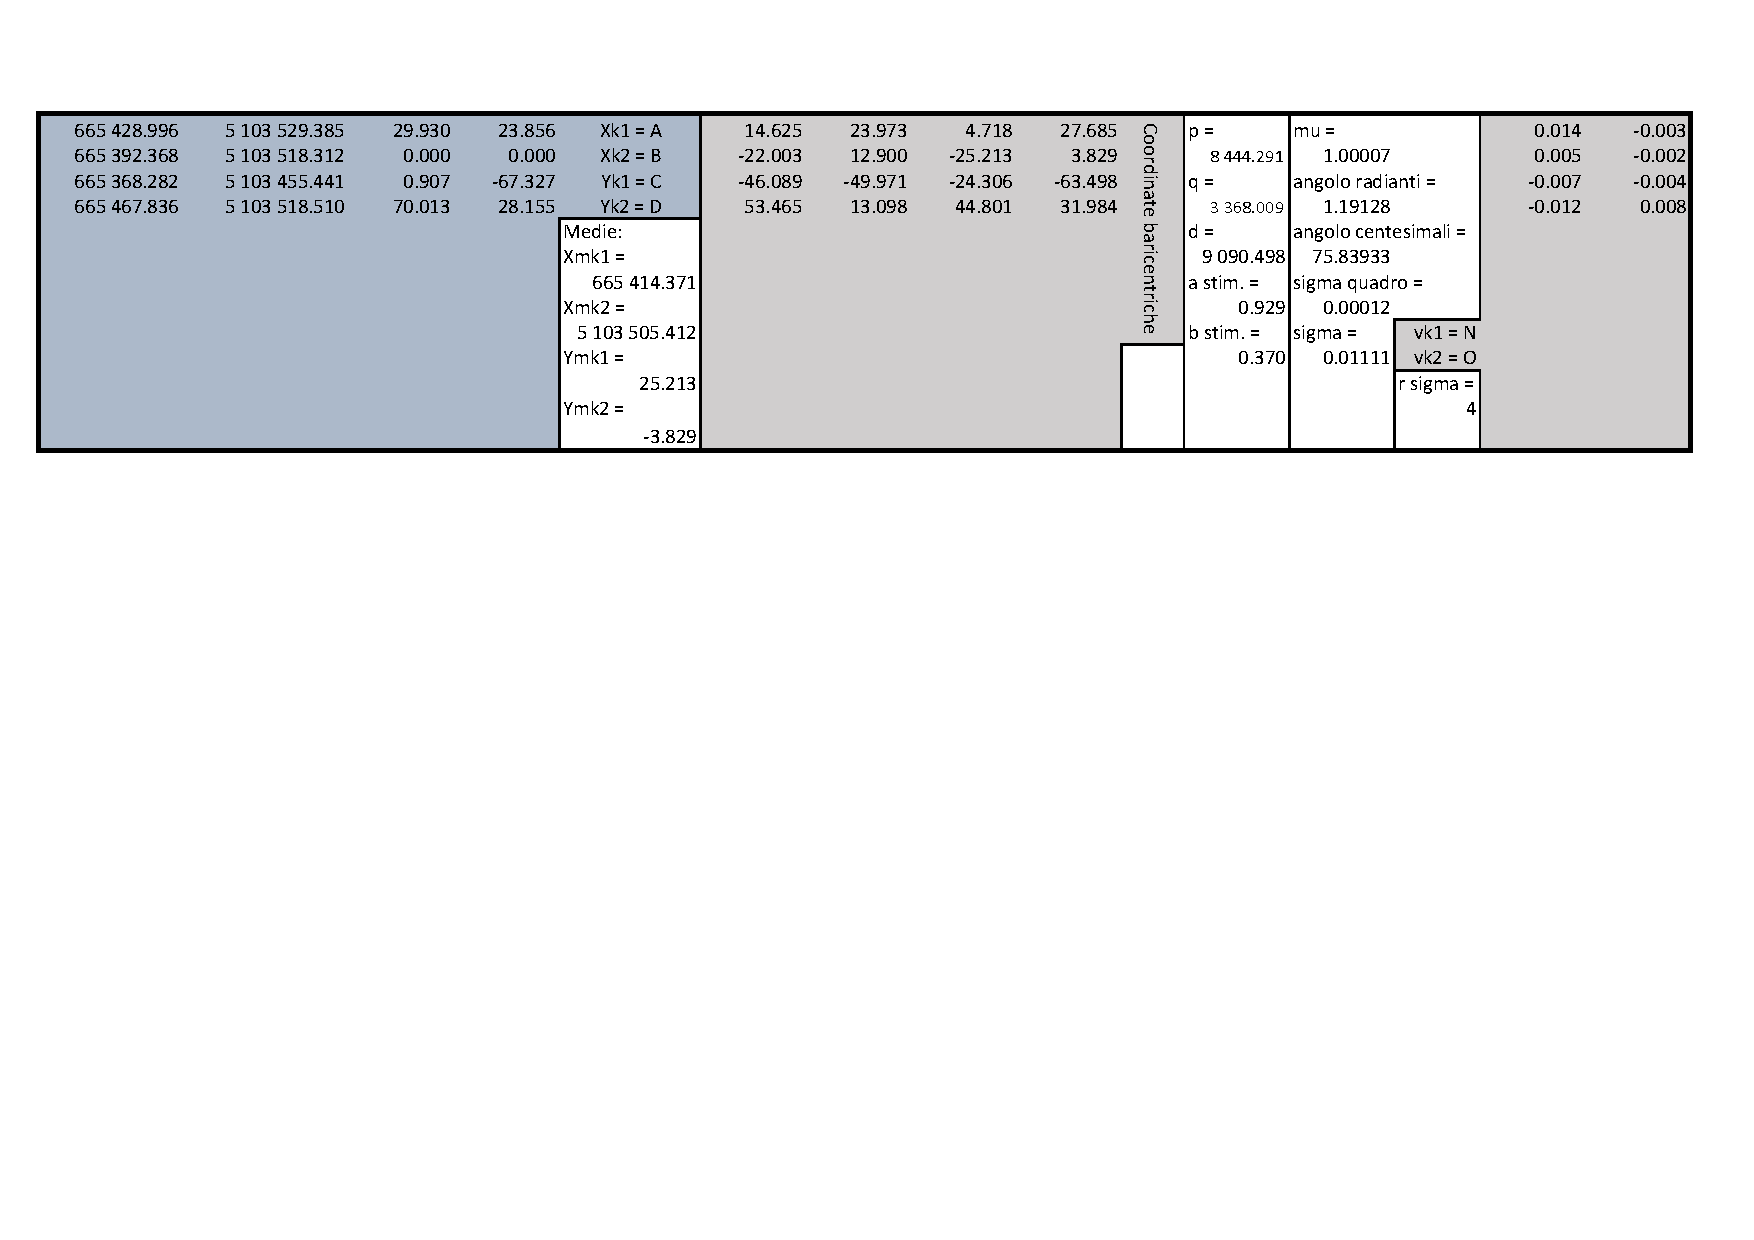
\includegraphics[width=16cm]{documents/rototraslazioneRilievo.pdf}
\caption{Schermata del foglio di calcolo con il quale è stata eseguita la rototraslazione del rilievo}
\end{figure}
	
%\vec: freccia (fisica)
%\boldsymbol: corsivo matematico
%\mathbf: tondo nero
